\documentclass[a4paper]{article}

\usepackage[polish]{babel}
\usepackage[utf8]{inputenc}
\usepackage{polski}
\usepackage{amsmath}
\usepackage{graphicx}
\usepackage[parfill]{parskip}
\usepackage{float}
\usepackage{multirow}

\title{Bezpieczeństwo usług sieciowych \\ --- laboratorium 1 --- \\ komunikator JSON + Diffie Hellman}

\author{Adrian Frydmański}

\date{\today}

\begin{document}
\maketitle

\section{Wstęp}
Celem laboratorium było stworzenie komunikatora (serwera i klienta) przesyłającego wiadomości w zdeklarowanych JSONach i ustalającego klucz szyfrowania przez algorytm Diffiego Hellmana.

\section{Opis projektu}
Zarówno klient jak i serwer napisane zostały przy użyciu języka Python 2.7.

\subsection{Sposób wykonania zadania}
Projekt składa się z dwóch skryptów: \texttt{server.py} i \texttt{client.py} oraz dodatkowego pliku \texttt{message.py} zawierającego kod współdzielony przez oba skrypty.

Wiadomości użyte w komunikacji wyglądają następująco:

\begin{figure}[H]
	\center
	\begin{tabular}{|l|l|l|}
		\hline 
		\textbf{Funkcja} & \textbf{Treść wiadomości} & \textbf{Kierunek} \\ 
		\hline 
		Żądanie wymiany kluczy & \texttt{\{ \char`\"request\char`\": \char`\"keys\char`\" \}} & $\uparrow$  \\ 
		\hline 
		Odpowiedź na żądanie & \texttt{\{ \char`\"p\char`\": 123, \char`\"g\char`\": 123 \}} & $\downarrow$ \\ 
		\hline 
		\multirow{ 2}{*}{Wymiana obliczonych a i b} & \texttt{\{ \char`\"a\char`\": 123 \}} & $\uparrow$ \\\cline{2-3} 
		& \texttt{\{ \char`\"b\char`\": 123 \}} & $\downarrow$ \\ 
		\hline 
		Ustawienie szyfrowania & \texttt{\{ \char`\"encryption\char`\": \char`\"none\char`\" \}} & $\uparrow$ \\ 
		\hline 
		Wymiana wiadomości & \texttt{\{ \char`\"msg\char`\": \char`\"\ldots\char`\", \char`\"from\char`\": \char`\"name\char`\" \}} & $\updownarrow$ \\ 
		\hline 
	\end{tabular} 
	\caption{Używane wiadomości}
\end{figure}

\subsubsection{Serwer}
Serwer należy uruchomić podając w argumencie numer portu (na przykład \texttt{./server.py 8000}).

Serwer uruchamia kilka wyspecjalizowanych wątków:
\begin{itemize}
	\item wątek główny --- odpowiada za nawiązanie połączenia. W przypadku połączenia przychodzącego tworzy wątek do obsługi go. Ponadto odpowiada za start wątku logera.
	\item loger --- służy do wyświetlania zdarzeń, rozwiązuje problem pisania na stdout z wielu wątków. Uruchamiany jeden na instancję serwera.
	\item wątek kliencki --- obsługuje połączenia przychodzące od klienta, uruchamiany dla każdego oddzielnie. Odpowiada za wymianę kluczy i ustawienie trybu szyfrowania. Uruchamia jeden ,,subwątek'' wysyłający wiadomości przychodzące od innych klientów.
	\item ,,subwątek'' kliencki --- zawiera kolejkę wiadomości do wysłania podłączonemu klientowi. Jeden na klienta. Odczytuje skolejkowane wiadomości do wysłania i umieszcza w gniazdku po uprzednim zaszyfrowaniu.
\end{itemize}

\subsubsection{Klient}
Klienta należy uruchomić podając w argumentach adres ip serwera i numer portu (na przykład \texttt{./client.py localhost 8000}). Ponadto można okreslić początkową metodę szyfrowania w kolejnych argumentach (\texttt{none}, \texttt{cezar} lub \texttt{xor}) oraz uruchomić w trybie testowania, dodając argunemt \texttt{bot}.

Klient na początku próbuje nawiązać połączenie z serwerem. Wysyła żądanie o liczby \texttt{p} i \texttt{g} z algorytmu Diffiego Hellmana, wylicza \texttt{A} czeka na wyliczoną przez serwer liczbę \texttt{B} i na ich podstawie oblicza klucz sesji.

Następnie wysyłana jest informacja o szyfrowaniu. Domyślne szyfrowanie to \texttt{none}, czyli jego brak --- wiadomości są widoczne dla wszystkich.

Klient uruchamia wątek wyświetlający przychodzace wiadomości. Odpowiada on za deszyfrację ich i działa niezależnie od wprowadzanego tekstu.

W pętli głównej odczytywane są wiadomości wpisane na standardowe wejście. W trybie testów wysyłana jest wiadomość testowa z kolejnym numerem co stały okres wynoszacy 2 sekundy.

Możliwa jest zmiana metody szyfrowania. Wystarczy wpisać w kliencie tę metodę poprzedzoną \texttt{@@@} (na przykład \texttt{@@@xor}, by zmienić szyfrowanie na xor). Wiadomości w tej postaci nie są wysyłane i są traktowane jako wiadomości sterujące.

\subsubsection{Szyfrowanie i wiadomości}
Szablony wiadomości, metody szyfrujące i deszyfrujące zostały umieszczone we współdzielonym pliku \texttt{message.py}.

Szyfrowanie i deszyfrowanie wygląda następująco:
\begin{itemize}
	\item XOR --- wykonanie operacji xor na każdym bajcie tekstu z najmłodszym bajtem klucza --- zarówno przy szyfrowaniu jak i deszyfrowaniu;
	\item Szyfr Cezara --- utworzenie słownika z przesunięciem o wartość klucza modulo połowa długości słownika (wynika to z faktu, że osobno przesuwane są małe i wielkie litery) i zamiana znaków zgodnie ze słownikiem. W przypadku deszyfrowania klucz ma wartość ujemną i operacja modulo daje jego dopełnienie do liczby będącej rozmiarem połowy słownika (liczby małych bądź wielkich liter).
\end{itemize}

\subsection{Użyte rozwiązania}
Wiadomości przesyłane między klientem, a serwerem są kodowane przy użyciu base64, by wpisany tekst nie naruszył struktury JSONa.

Liczby \texttt{p} i \texttt{g} są generowane dzięki funkcji \texttt{Crypto.Util.number.getPrime()}.

\section{Testy}
Poniżej opisano wykonane testy mające na celu sprawdzenie poprawności działania skryptów.

\subsection{Testy jednostkowe}
Przeprowadzono testy jednostkowe z użyciem wbudowanego w Pythona \texttt{unittest}. Uruchamianie testów jednostkowych odbywa się poprzez uruchomienie skryptu \texttt{tests.py}. Testy jednostkowe sprawdzają poprawność szyfrowania i deszyfrowania wiadomości.

\begin{figure}[H]
	\center
	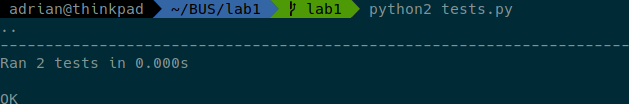
\includegraphics[width=.6\textwidth]{img/tests.png}
	\caption{Uruchamianie testów jednostkowych.}
\end{figure}

\subsection{Przesyłanie i odbieranie wiadomości}
Podstawowym testem jest sprawdzeniepoprawności wysyłania i odbierania wiadomości przez kilenta i serwer. Test został wbudowany jako funkcjonalność klienta. Należy uruchomić go z argumentem \texttt{bot}. W wyniku tego klient zacznie wysyłać wiadomości z kolejnymi numerami do serwera. Serwer odbierze je i roześle pozostałym podłączonym klientom.

\begin{figure}[H]
	\center
	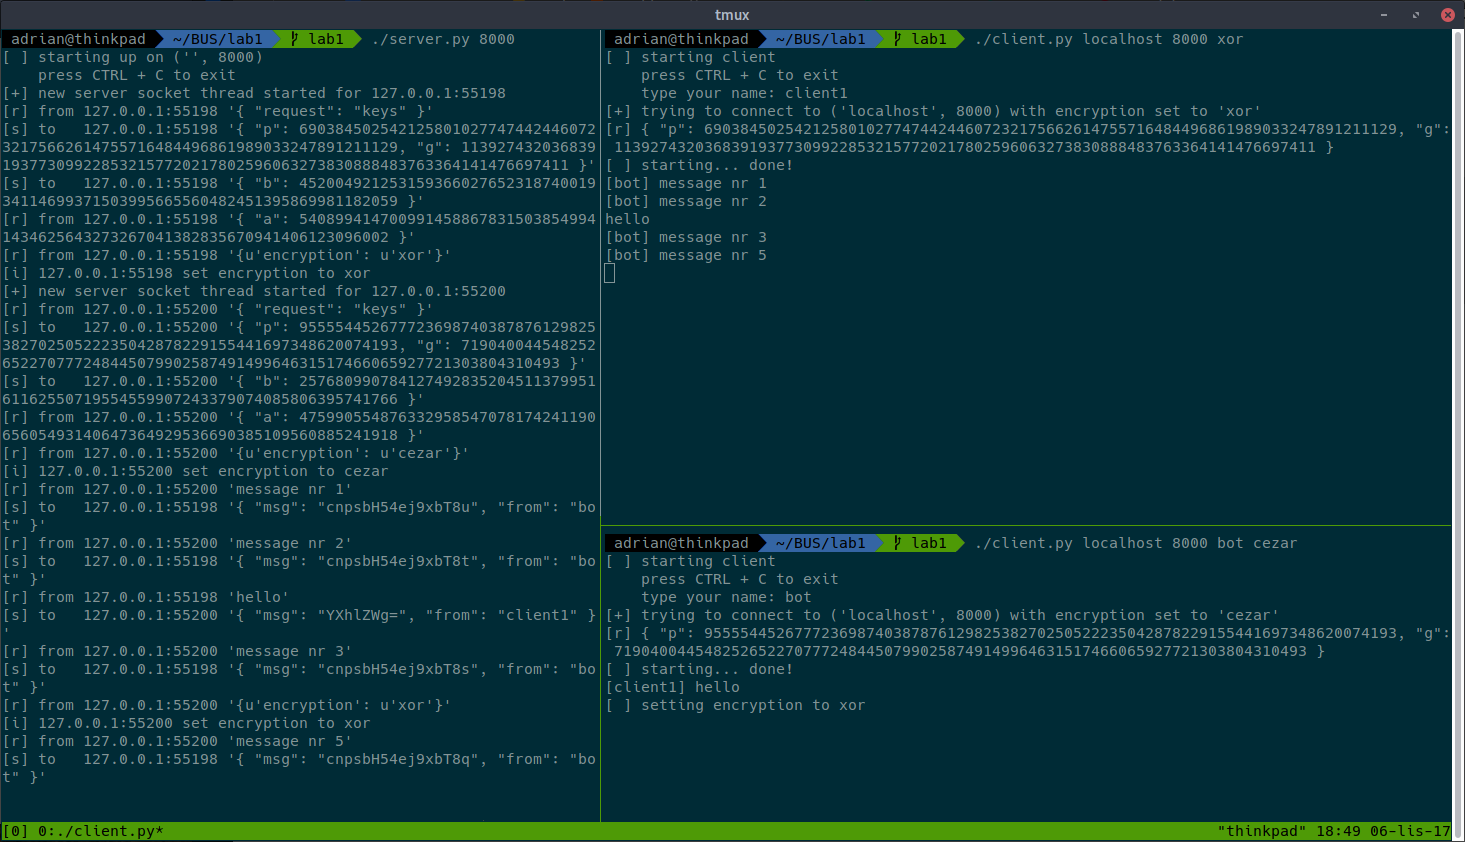
\includegraphics[width=.8\textwidth]{img/testbot.png}
	\caption{Testy --- uruchamianie i zmiana szyfrowania przez bota}
\end{figure}

\begin{figure}[H]
	\center
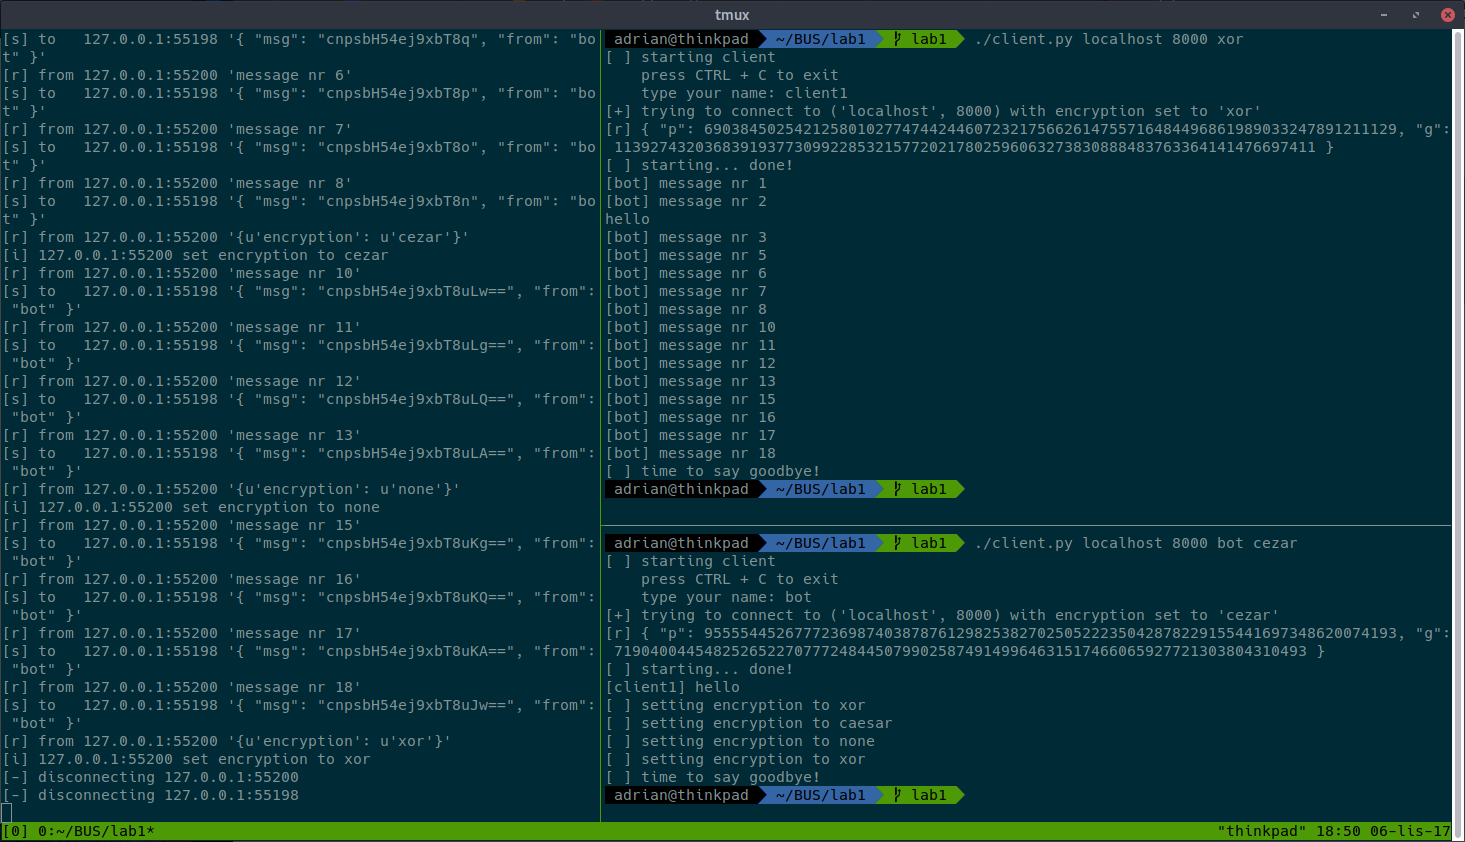
\includegraphics[width=.8\textwidth]{img/testbot2.png}
\caption{Testy --- zamykanie klientów}
\end{figure}

Po uruchomieniu serwera uruchamiani są kolejni klienci (z klientem w trybie testów na końcu). Widać nawiązywanie połączenia każdego z nich w logach serwera, a po uruchomieniu ostatniego wysłane 4 wiadomości z kienta \texttt{bot}.

Taki sam test przeprowadzono uruchamiając serwer i klientów na różnych urządzeniach.

\subsection{Wireshark}
Dzięki oprogramowaniu Wireshark możliwy jest podgląd przesyłanych pakietów pomiędzy klientami, a serwerem.

\begin{figure}[H]
	\center
	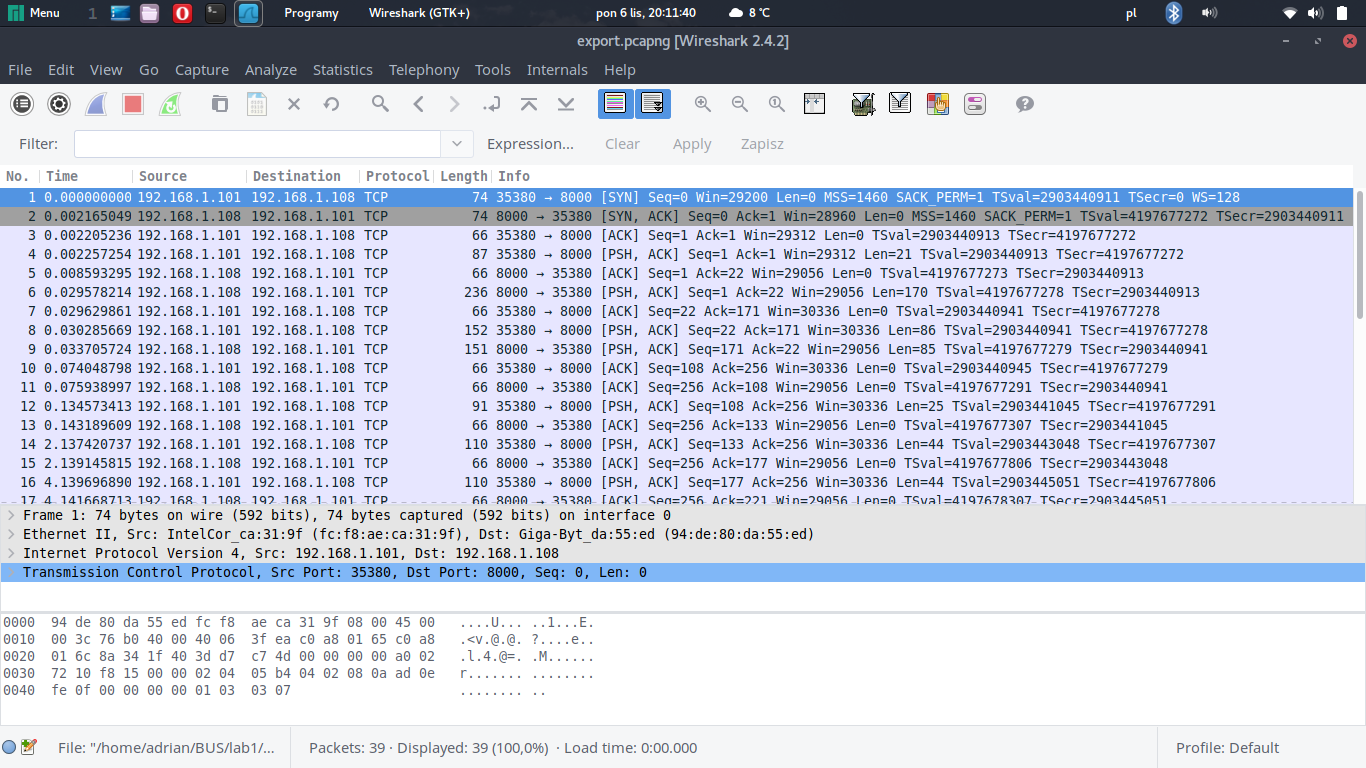
\includegraphics[width=.8\textwidth]{img/1-handshake.png}
	\caption{Wireshark --- handshake}
\end{figure}

\begin{figure}[H]
	\center
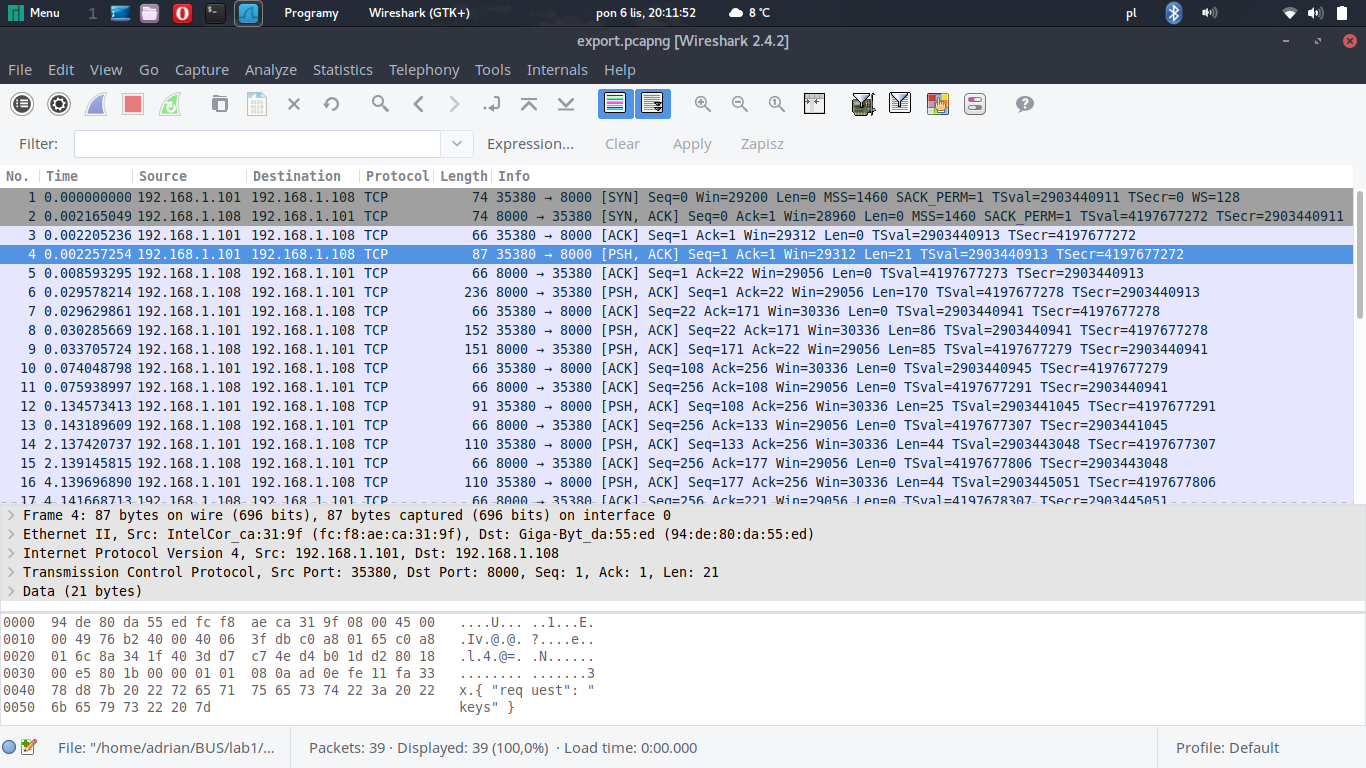
\includegraphics[width=.8\textwidth]{img/2-request.png}
\caption{Wireshark --- żądanie wymiany kluczy}
\end{figure}

\begin{figure}[H]
	\center
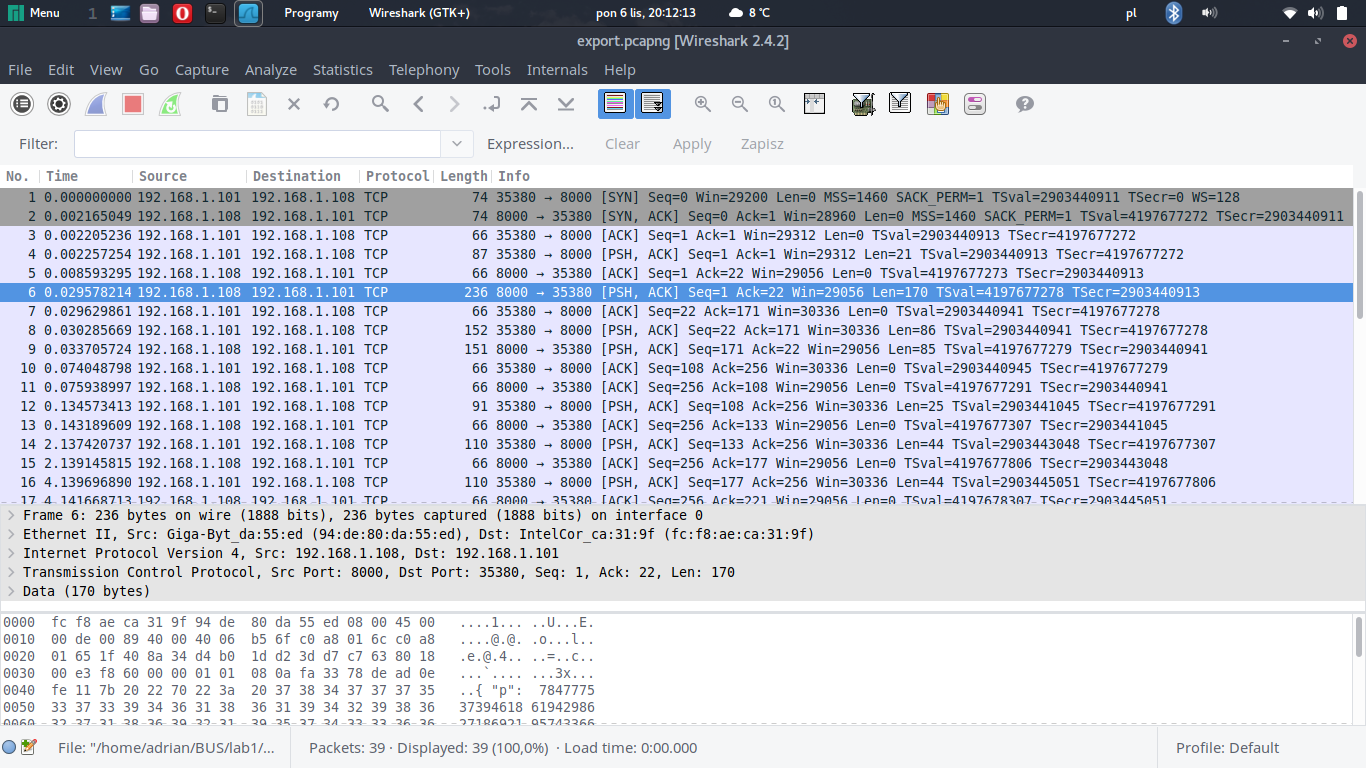
\includegraphics[width=.8\textwidth]{img/3-pq.png}
\caption{Wireshark --- liczby \texttt{p} i \texttt{q} od serwera}
\end{figure}

\begin{figure}[H]
	\center
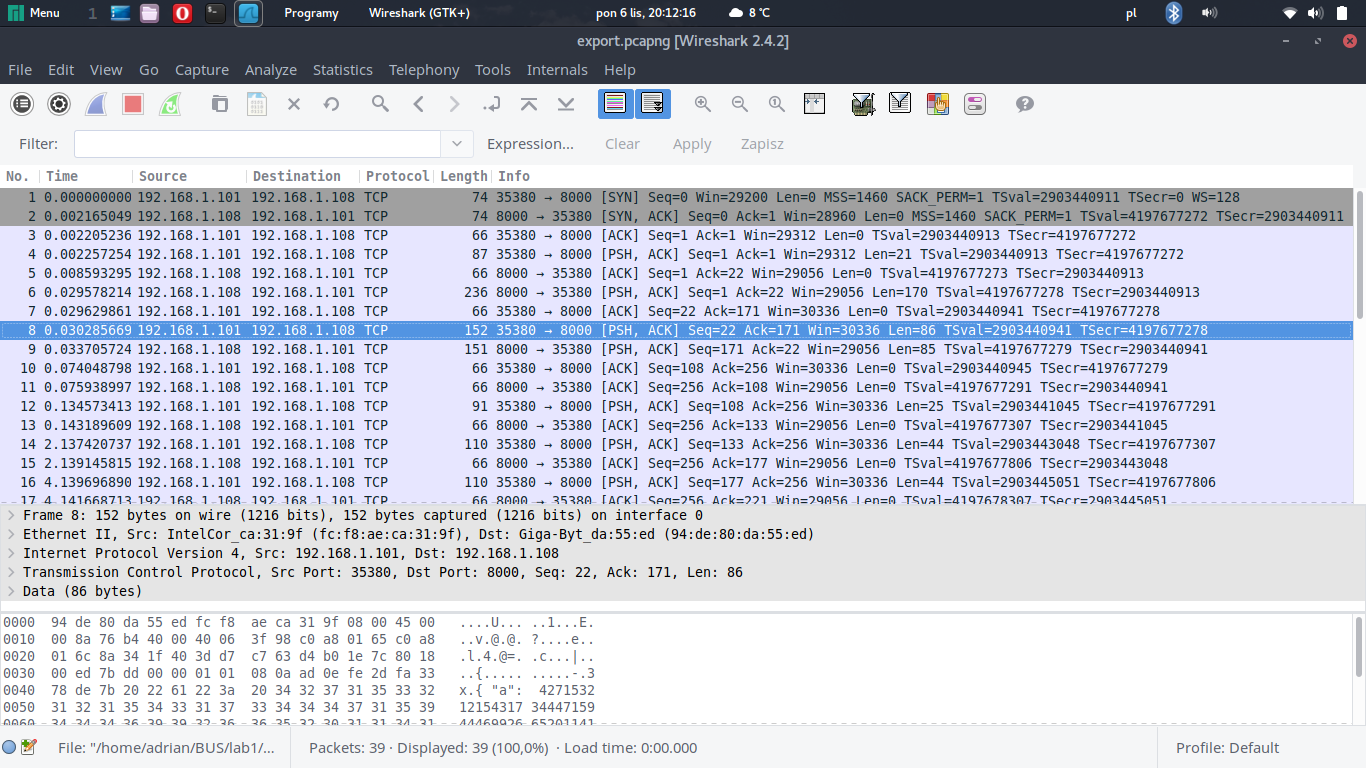
\includegraphics[width=.8\textwidth]{img/4-a.png}
\caption{Wireshark --- wysłanie liczby \texttt{A} do serwera}
\end{figure}

\begin{figure}[H]
	\center
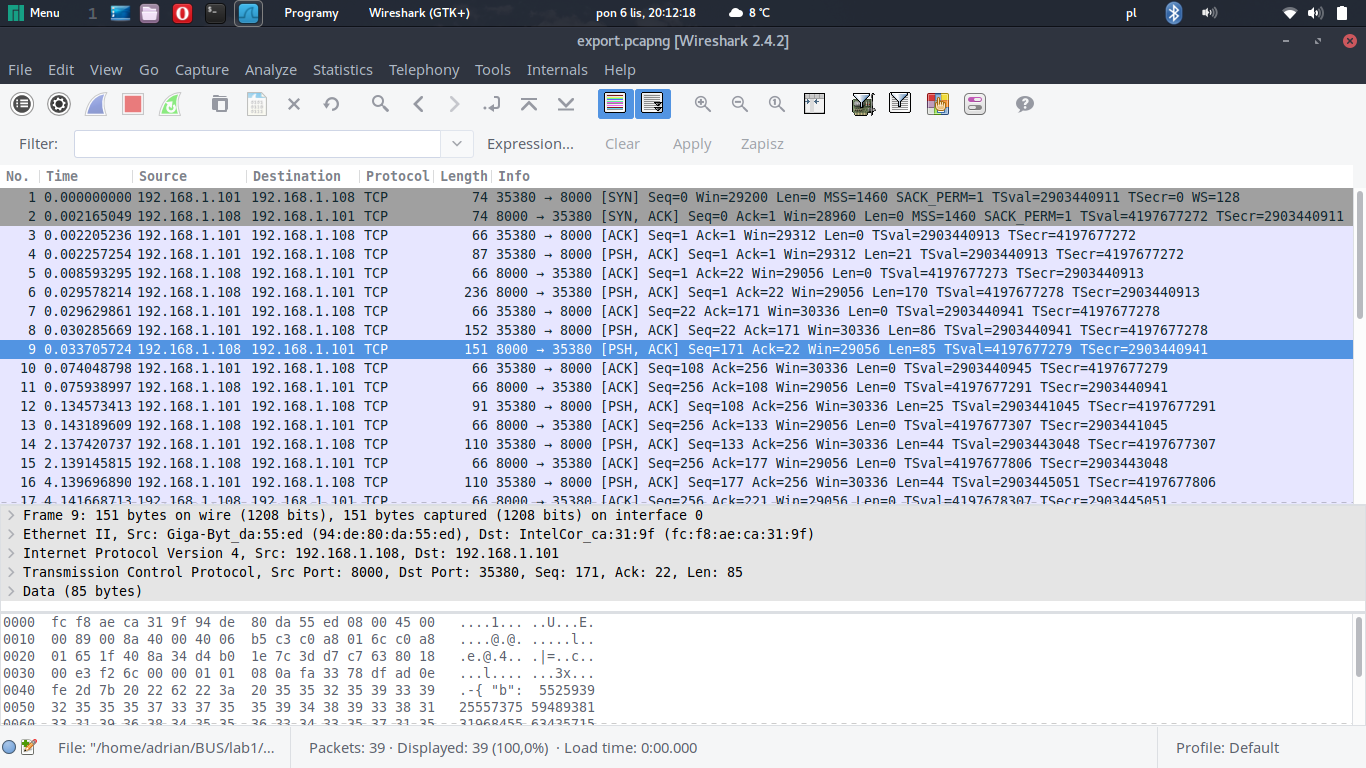
\includegraphics[width=.8\textwidth]{img/5-b.png}
\caption{Wireshark --- odebranie liczby \texttt{B} z serwera}
\end{figure}

\begin{figure}[H]
	\center
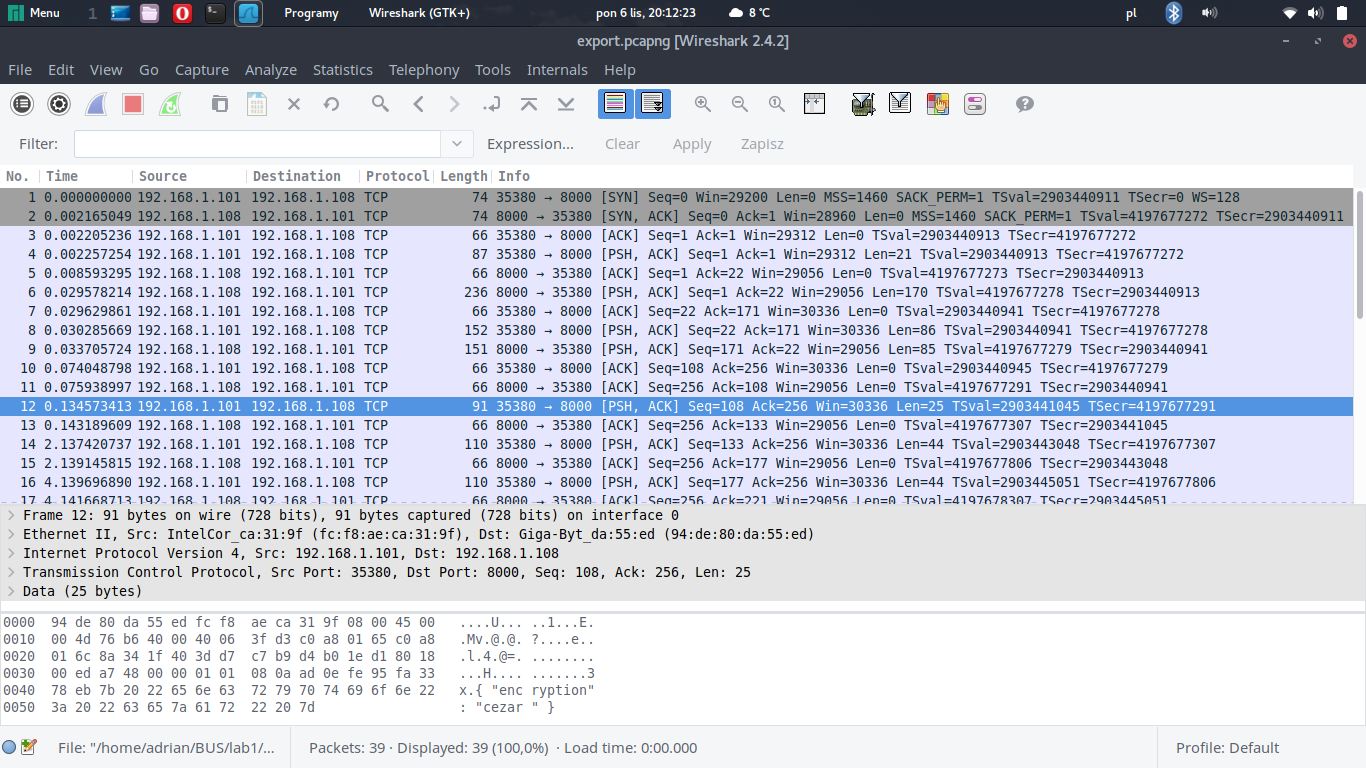
\includegraphics[width=.8\textwidth]{img/6-enc.png}
\caption{Wireshark --- wysłanie informacji o szyfrowaniu}
\end{figure}

\begin{figure}[H]
	\center
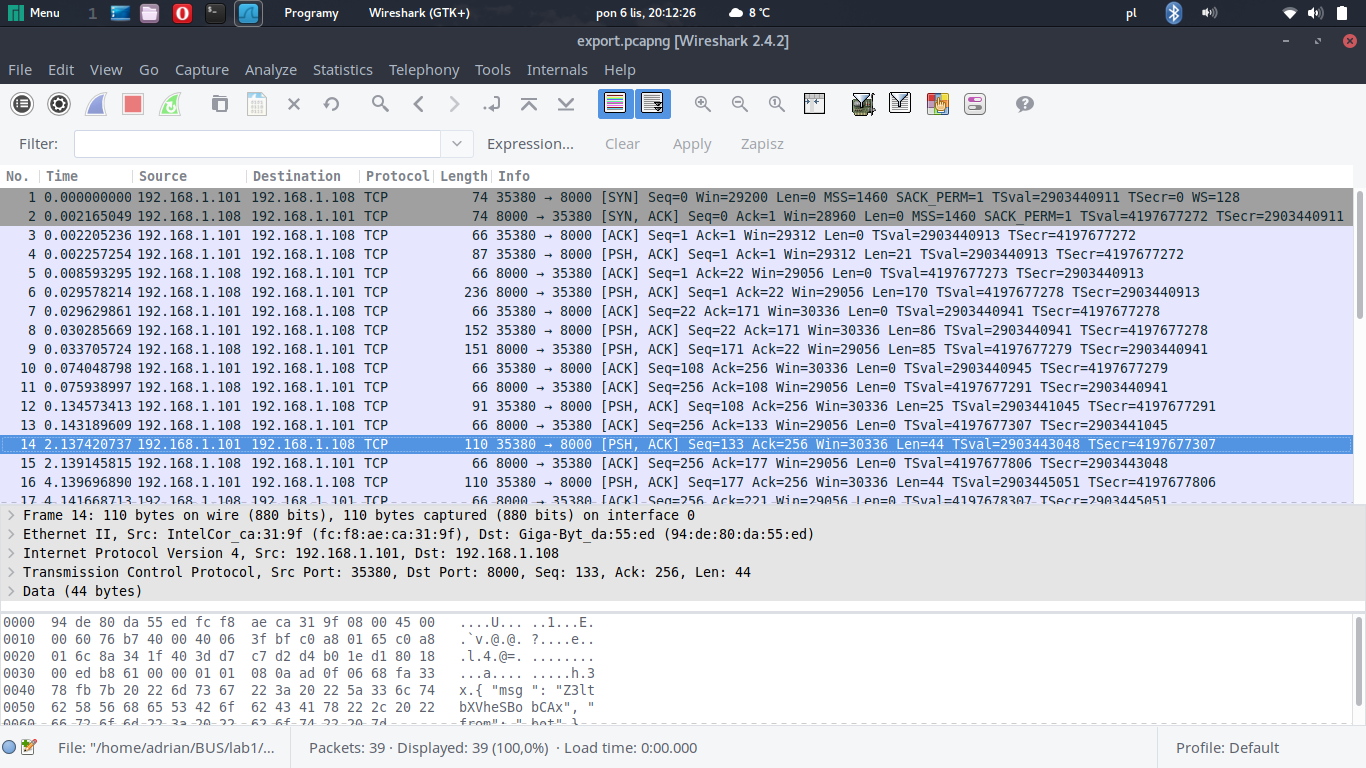
\includegraphics[width=.8\textwidth]{img/7-msg.png}
\caption{Wireshark --- wysłanie wiadomości}
\end{figure}

Można zauważyć, że przesyłana wiadomość jest zakodowana, a po zdekodowaniu jej z base64 nadal trzeba ją odszyfrować zgodnie z przyjętym szyfrowaniem.

\section{Wnioski}
Prosty komunikator uruchamiany w terminalu mógłby zostać rozbudowany o graficzne międzymordzie użytkownika. W prosty sposób rozwiązałoby to problem usuwania wpisywanej wiadomości podczas otrzymywania innej z serwera i wyświetlania jej na ekranie. W konsoli wymagałoby to użycia dodatkowych bibliotek (jak \texttt{Curses}).


\end{document}